\chapter{Descripción}\label{chap:descripcion}

La investigación con usuarios aporta indicios sobre dificultades de seguimiento e interpretación de inversiones. Con esos indicios se delimitan el problema, la solución y sus requerimientos. La sección distingue lo relevado de las hipótesis de diseño y de lo que no llegó a validarse.

\section{Investigación con usuarios}\label{sec:user-research}

El relevamiento combina una encuesta y entrevistas semiestructuradas. La encuesta aporta resultados agregados; las entrevistas exploran prácticas y motivos. La consulta al tutor se considera orientación académica y queda excluida de la muestra de usuarios para evitar el sesgo derivado de su participación en el Proyecto.

\subsection{Encuesta}\label{subsec:encuesta}

El formulario \textit{Encuesta sobre análisis y gestión de inversiones} reúne 190 respuestas entre el 24 de mayo y el 14 de agosto de 2026. Su difusión comprende redes sociales, grupos vinculados con finanzas y contactos directos. El muestreo es no probabilístico por conveniencia: los resultados describen a los participantes y no estiman la demanda del conjunto de inversores argentinos. El Anexo~\ref{annex:user-research} reúne el cuestionario aplicado y las frecuencias documentadas.

\subsubsection{Perfil y límites de la muestra}

La Figura~\ref{fig:encuesta-perfil} muestra que la muestra reúne inversores activos, personas con seguimiento ocasional y personas que todavía no invierten. El segmento activo comprende 85 participantes, mientras que 48 no invierten. Los tres grupos se tratan por separado, porque no comparten experiencia de uso ni necesidades.

La edad se concentra entre 18 y 34 años (135 de 190 participantes). La encuesta no releva ubicación geográfica, y sus frecuencias marginales no indican cuántos inversores activos operan en varias plataformas. El contexto argentino proviene del diseño del Proyecto y de las menciones de instrumentos locales, no de una residencia relevada.

\begin{figure}[ht]
\centering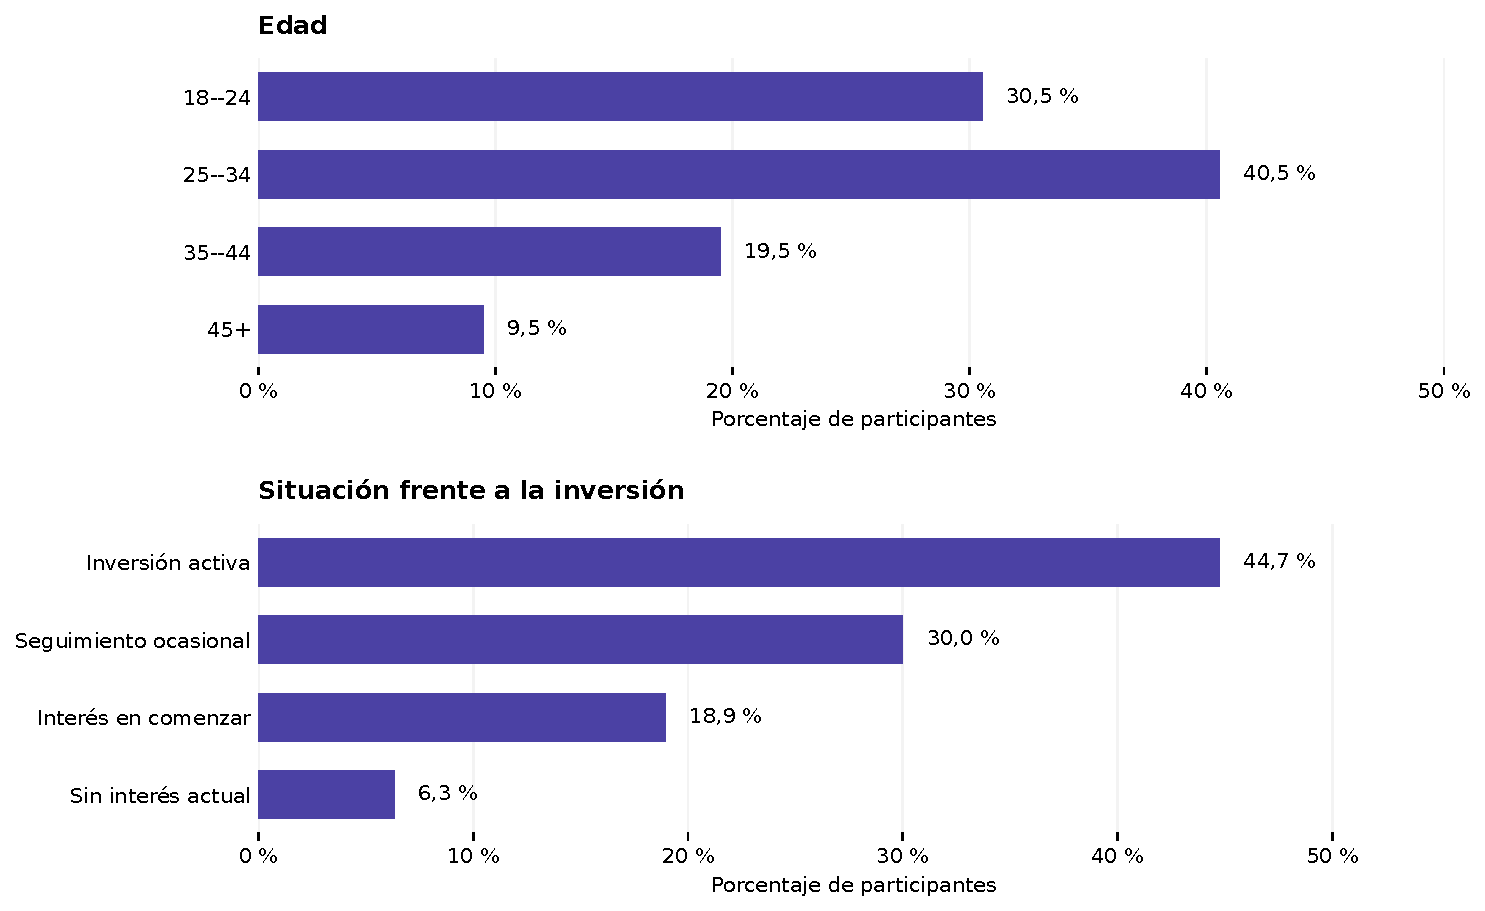
\includegraphics[width=\textwidth]{figures/encuesta_perfil}
\caption{Perfil de los participantes (N=190). Fuente: elaboración propia.}\label{fig:encuesta-perfil}
\end{figure}

\subsubsection{Seguimiento y dificultades}

Las formas de seguimiento incluyen aplicaciones de cada plataforma y planillas propias. La preferencia por una visión consolidada y las dificultades de interpretación orientan el diseño hacia una carga única y un resumen común. La pregunta sobre activos mezcla tenencias actuales e interés futuro; por eso sus respuestas se leen como indicio y no como composición real de las carteras.

La Figura~\ref{fig:encuesta-dificultades} compara las dificultades sin repetir todas las distribuciones del anexo. La consolidación y el tiempo de investigación destacan junto con la comprensión de la diversificación y la exposición. Estas respuestas justifican estudiar el problema; si el prototipo lo resuelve es una pregunta de la evaluación.

\begin{figure}[ht]
\centering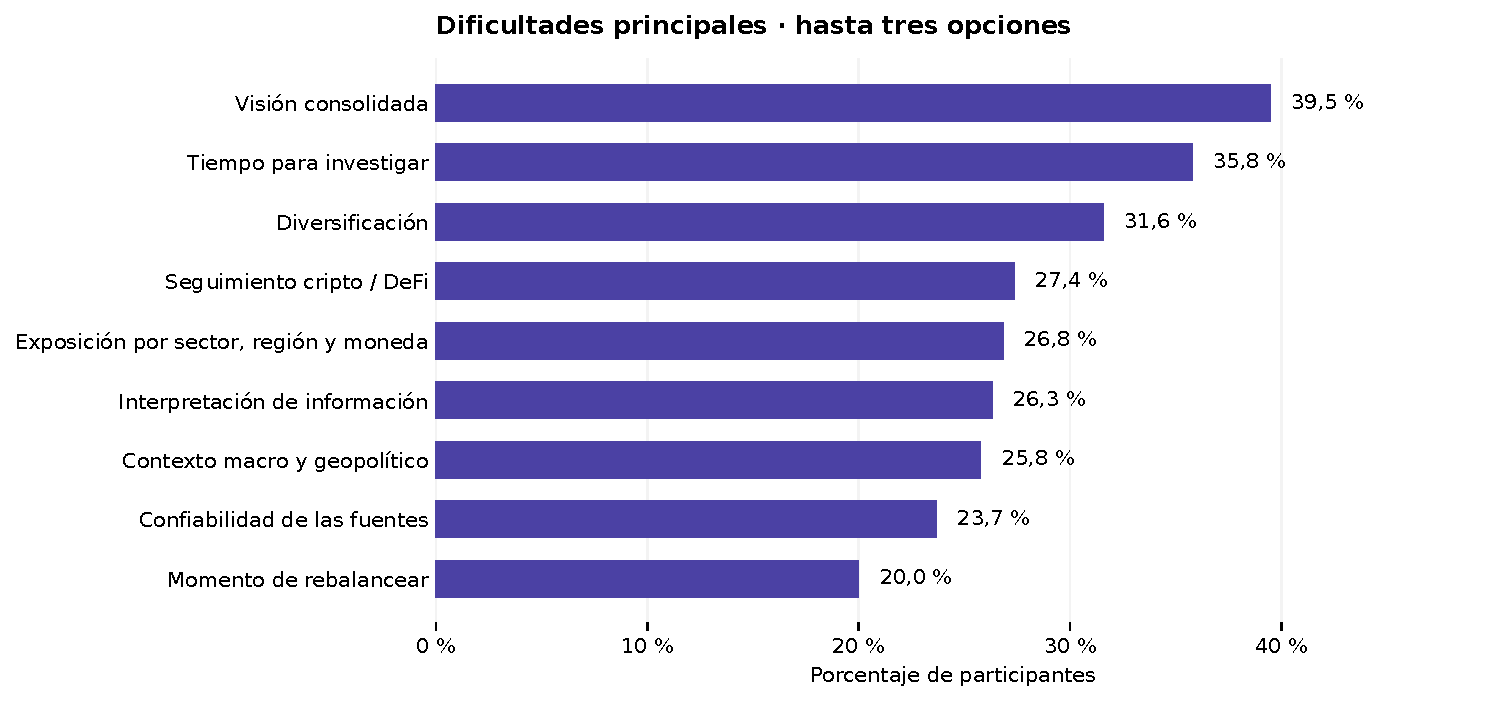
\includegraphics[width=\textwidth]{figures/encuesta_dificultades}
\caption{Dificultades de análisis y seguimiento (N=190). Fuente: elaboración propia.}\label{fig:encuesta-dificultades}
\end{figure}

\subsubsection{Prioridades e interés en la propuesta}

La Figura~\ref{fig:encuesta-funcionalidades} presenta las prioridades declaradas. La vista consolidada, el análisis de exposición y la explicación de observaciones orientan el núcleo funcional. Las preguntas de selección múltiple admiten hasta tres opciones; sus porcentajes se calculan sobre los 190 participantes, por lo que no suman 100\,\%.

\begin{figure}[ht]
\centering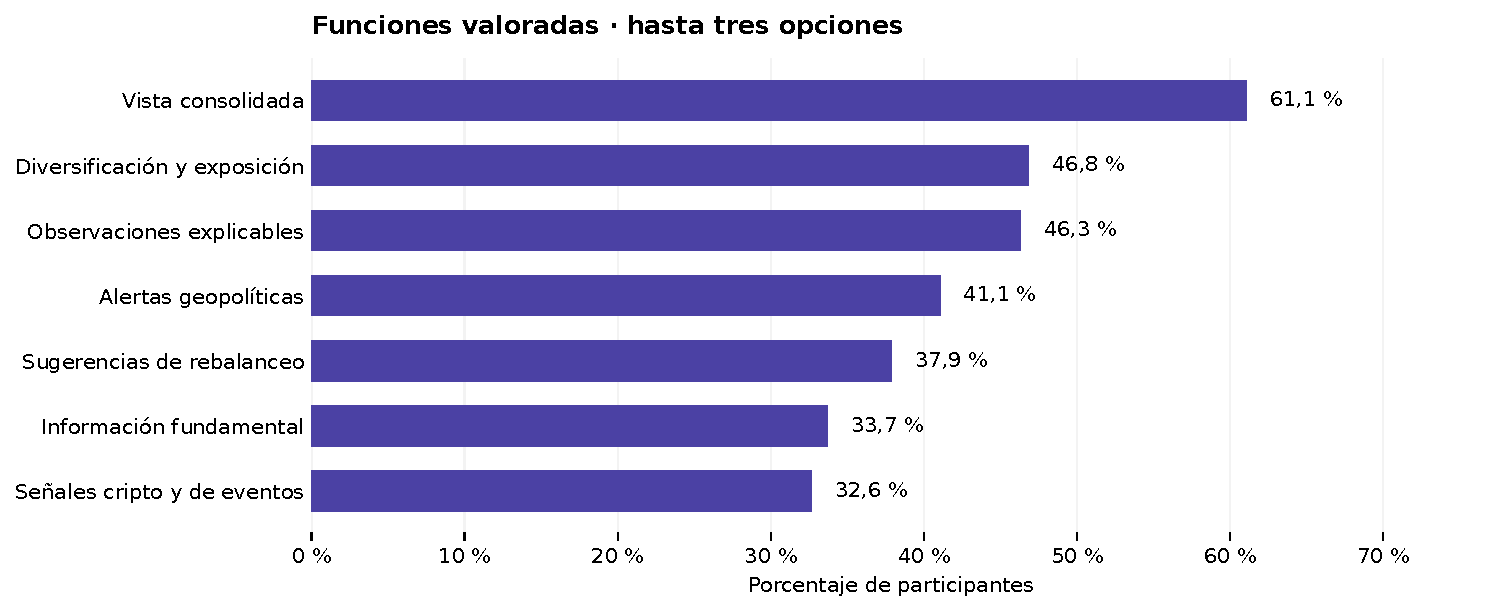
\includegraphics[width=\textwidth]{figures/encuesta_funcionalidades}
\caption{Prioridades funcionales declaradas (N=190). Fuente: elaboración propia.}\label{fig:encuesta-funcionalidades}
\end{figure}

La pregunta sobre interés describe expresamente una plataforma web. La Figura~\ref{fig:encuesta-interes} muestra una concentración de respuestas en niveles altos y una preferencia por acceso gratuito con funciones pagas. Ese interés es declarado: la adopción, el pago y la valoración de una aplicación móvil quedan por medir.

\begin{figure}[ht]
\centering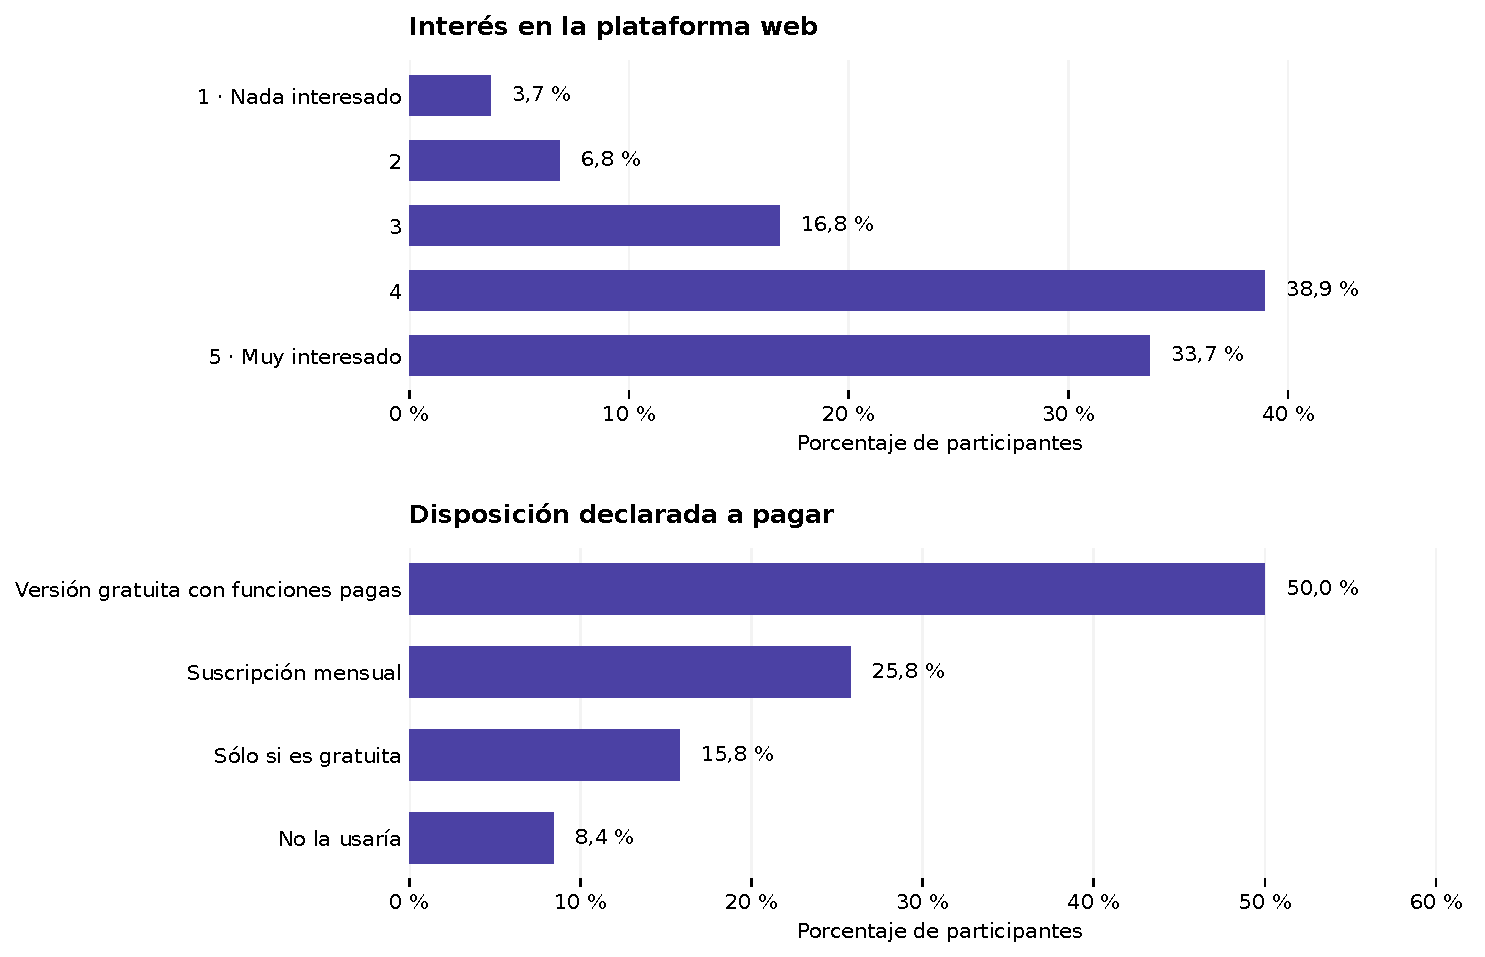
\includegraphics[width=\textwidth]{figures/encuesta_interes}
\caption{Interés en la plataforma web y disposición a pagar (N=190). Fuente: elaboración propia.}\label{fig:encuesta-interes}
\end{figure}

Existen solapamientos entre las preguntas 13 y 14 sobre explicación, entre las preguntas 6 y 15 sobre herramientas y entre las preguntas 11 y 13 sobre señales. Se interpretan como perspectivas complementarias del mismo tema, no como corroboraciones independientes. El 60,0\,\% que asigna importancia alta a la explicación y el 46,3\,\% que la selecciona entre tres funciones prioritarias responden consignas diferentes.

Los porcentajes desagregados por actividad inversora y las combinaciones de activos solo pueden auditarse con registros individuales. Las tablas agregadas no reconstruyen esos cruces, por lo que no se presentan como resultados verificados.

\subsubsection{Lectura cualitativa y consecuencias para el diseño}

La pregunta 16 es abierta: \enquote{¿Qué sentís que le falta a las herramientas que usás hoy para analizar mejor tu portafolio?}. De las 190 respuestas, 163 son sustantivas y 27 no aportan contenido (guiones, \enquote{no sé} o \enquote{no uso}). El Anexo~\ref{annex:user-research} las transcribe completas en la Tabla~\ref{tab:encuesta-abierta} y resume su codificación temática en la Tabla~\ref{tab:encuesta-temas}; una respuesta puede corresponder a más de un tema. Los temas más frecuentes son el contexto argentino, es decir, la inflación, el tipo de cambio y los instrumentos locales (46 respuestas); la consolidación e integración entre plataformas (39); las noticias, las alertas y el efecto del contexto sobre la cartera (34), y la carga y actualización automáticas (23). Siguen el lenguaje accesible (18), la exposición real y la composición de los fondos (18), los criptoactivos (18) y la explicación de las recomendaciones (14). Un participante lo resume así: \enquote{Tengo cuenta en Balanz en IOL y en Lemon y cada uno me muestra sus números pero nunca veo el cuadro completo}; otro pide \enquote{entender el razonamiento detrás} de lo que se le sugiere. La codificación es propia y exploratoria: la hizo el equipo con reglas de palabras clave revisadas respuesta por respuesta, sin un segundo codificador.

De allí derivan tres decisiones: una vista común de posiciones, indicadores con definiciones visibles y evidencia vinculada a cada observación. La ganancia ajustada por inflación y la conexión automática con los intermediarios, que varias respuestas piden, quedan fuera del alcance. Si esas decisiones mejoran la comprensión se evalúa con tareas concretas, no con el interés declarado en la encuesta.

\subsection{Entrevistas}\label{subsec:entrevistas}

Se entrevistó a tres inversores minoristas ajenos al equipo y a la tutoría: Tadeo Pinque, Fabricio Sabattoli y Octavio Antunes. Las conversaciones se realizaron el 22 de octubre de 2026 por videollamada, con la guía de cinco preguntas del Anexo~\ref{annex:entrevistas}, donde figuran los perfiles; las transcripciones completas están en los Anexos~\ref{annex:entrevista-tadeo}, \ref{annex:entrevista-fabricio} y~\ref{annex:entrevista-octavio}. Los párrafos siguientes resumen cada conversación y citan sus pasajes centrales.

Tadeo Pinque sigue acciones y ETFs desde la aplicación con la que compra y, a fin de mes, usa una herramienta de IA \enquote{para analizar los resultados y validar en qué podría mejorar}. Intenta concentrarse en una plataforma, pero termina usando varias porque hay acciones que \enquote{no se pueden comprar desde Argentina} o criptomonedas que no están en ciertos brokers. Su última compra, una acción de semiconductores tras una caída, se apoyó en análisis de mercado y chats con IA; le hubiera gustado que la misma plataforma le diera información sobre la empresa antes de decidir. Las opiniones de otros inversores que muestran algunas plataformas las toma \enquote{como un parámetro}, pero las contrasta con su propia investigación. A la herramienta ideal le pide que le indique cómo reequilibrar la cartera según su estilo: si tiene muchas acciones vinculadas a IA, que le sugiera incorporar otro tipo de empresas para que \enquote{en caso de que el mercado castigue fuerte no tenga mucha pérdida}. Ese pedido corresponde a la concentración sectorial y a los escenarios adversos del diseño; la sugerencia de instrumentos concretos queda fuera del alcance informativo.

Fabricio Sabattoli tiene casi todas sus inversiones en Balanz y el resto en Binance, y consolida en Yahoo Finance, donde \enquote{bonos, letras o fondos} locales no se pueden cargar. Se informa en X y Yahoo Finance y usa Claude como apoyo; no siente que le falte información. Nunca recibió una recomendación formal, pero observa que muchos posts en X \enquote{indirectamente se inclinan hacia una recomendación}, que tiende a aceptar cuando refuerzan su posición, y advierte que quien publica una recomendación \enquote{ya tomó una posición previa} y el efecto \enquote{ya esté desencadenado en el precio}. A la herramienta ideal le pediría el sentimiento sobre un activo para \enquote{ver ambos lados de la moneda}. Su aporte específico es la dificultad de representar instrumentos locales en consolidadores globales y la demanda de contexto con fuentes contrastables, que orienta la presentación de señales con procedencia.

Octavio Antunes describe un seguimiento \enquote{bastante manual}: aplicaciones de cada broker (Interactive Brokers, Binance y un broker local), Yahoo Finance, Google Finance y TradingView para precios y noticias, y un Excel para registrar lo invertido. Su problema principal es la dispersión: cada aplicación muestra su propio rendimiento y \enquote{ninguna me permite entender fácilmente cómo está distribuida toda mi cartera}; calcular qué porcentaje tiene en acciones, ETFs o cripto lo hace a mano. En su última decisión, aumentar la exposición al mercado estadounidense con un ETF del S\&P 500, analizó rendimiento histórico, noticias y tasas, pero le faltó saber \enquote{si estaba demasiado concentrado en determinados sectores o mercados} y una comparación de escenarios sobre cómo la compra modificaría la diversificación. Las alertas que recibió le resultaron demasiado generales: un aviso de caída del 5\,\% no explica si la causa es un resultado de la empresa, una noticia política o el mercado general, por lo que las usa solo como punto de partida. Confiaría más en una recomendación si pudiera \enquote{entender claramente qué información se utilizó para generarla, qué riesgo considera y cómo se relaciona con mi cartera particular}. Pide integrar todas sus inversiones sin transferir activos, analizar composición y concentración, relacionar acontecimientos económicos y políticos con sus tenencias y avisar solo cuando ocurra algo relevante. Rechaza que la herramienta compre o venda sin su autorización, que prometa rendimientos garantizados o que recomiende sin explicar fundamentos: busca \enquote{tomar decisiones más informadas} sin que la herramienta reemplace su criterio. Esta entrevista es la que describe con más precisión el problema que el Proyecto delimita y coincide, punto por punto, con RF2, RF4, RF5, RF6, RF8, RF12 y RNF8.

La síntesis de las tres conversaciones muestra tres temas recurrentes. Primero, la cartera está repartida entre varias plataformas en los tres casos y la consolidación es manual (Yahoo Finance, Excel) o inexistente. Segundo, los tres desconfían de las recomendaciones sin fundamento: Fabricio por el interés previo de quien recomienda, Tadeo porque valida con investigación propia y Octavio porque las alertas no explican la causa; los tres piden entender qué datos y qué riesgo hay detrás de una sugerencia. Tercero, la IA ya forma parte de su rutina como apoyo de lectura (Tadeo y Fabricio), no como decisor. Las diferencias también informan el diseño: Tadeo pide sugerencias de reequilibrio, Fabricio sentimiento con ambos lados y Octavio composición, concentración y contexto; los dos últimos pedidos están en el alcance, el primero solo en su parte descriptiva. Tres entrevistas por conveniencia no alcanzan saturación temática, pero la coincidencia de los tres en dispersión y en explicabilidad respalda las decisiones de carga única, exposición calculada y evidencia por observación. No se sabe si los entrevistados respondieron la encuesta, por lo que los dos instrumentos no se tratan como independientes.

\subsection{Personas usuarias}\label{subsec:user-persona}

Se definen tres arquetipos de diseño: inversor activo, inversor con seguimiento ocasional y persona interesada en comenzar. Las Figuras~\ref{fig:persona-activo}, \ref{fig:persona-ocasional} y~\ref{fig:persona-principiante}, reunidas en el Anexo~\ref{annex:personas}, distinguen la base empírica de las hipótesis. Los nombres y retratos esquemáticos son ficticios; ciudad, profesión, ingresos y combinaciones de activos figuran como supuestos, no como datos relevados.

Martín representa el seguimiento activo y la necesidad de inspeccionar exposiciones; Clara representa la revisión ocasional y la lectura de un resumen comprensible; Alex representa el aprendizaje inicial y la necesidad de comprender términos antes de analizar una cartera de ejemplo. Estas personas guían los escenarios de evaluación. Las frecuencias de las categorías de inversión justifican los tres segmentos; los comportamientos particulares de cada arquetipo son hipótesis de diseño.

\subsection{Análisis FODA}\label{subsec:foda}

La Figura~\ref{fig:foda} relaciona decisiones internas y condiciones externas después de presentar los resultados de la encuesta. La valoración es cualitativa y corresponde al diseño del Proyecto.
\begin{figure}[ht]\centering
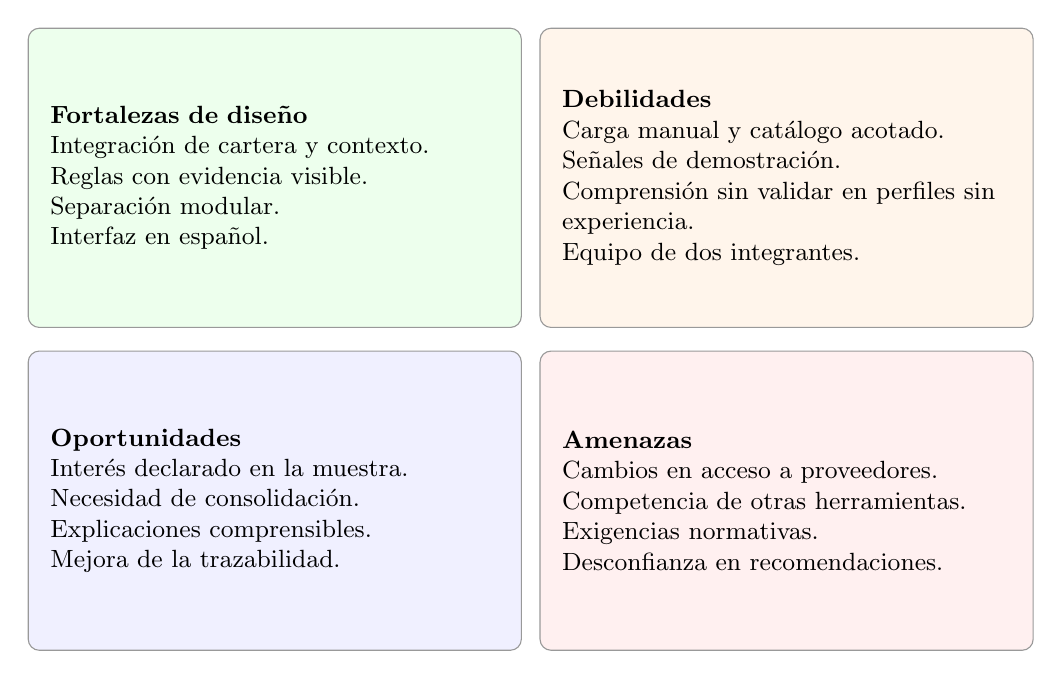
\begin{tikzpicture}[q/.style={draw=black!40,rounded corners,text width=5.7cm,minimum height=3.8cm,align=left,inner sep=8pt,font=\small,anchor=north west}]
\node[q,fill=green!7] at (0,0) {\textbf{Fortalezas de diseño}\\Integración de cartera y contexto.\\Reglas con evidencia visible.\\Separación modular.\\Interfaz en español.};
\node[q,fill=orange!8] at (6.5,0) {\textbf{Debilidades}\\Carga manual y catálogo acotado.\\Señales de demostración.\\Comprensión sin validar en perfiles sin experiencia.\\Equipo de dos integrantes.};
\node[q,fill=blue!6] at (0,-4.1) {\textbf{Oportunidades}\\Interés declarado en la muestra.\\Necesidad de consolidación.\\Explicaciones comprensibles.\\Mejora de la trazabilidad.};
\node[q,fill=red!6] at (6.5,-4.1) {\textbf{Amenazas}\\Cambios en acceso a proveedores.\\Competencia de otras herramientas.\\Exigencias normativas.\\Desconfianza en recomendaciones.};
\end{tikzpicture}
\caption{Análisis FODA del Proyecto. Fuente: elaboración propia.}\label{fig:foda}
\end{figure}


La integración de información y la evidencia inspeccionable son las fortalezas de diseño. La carga manual, el catálogo acotado y la combinación de señales en vivo con datos de demostración son las debilidades del prototipo. El interés declarado en la encuesta abre una oportunidad de investigación; la demanda comercial queda por verificar. La dependencia de proveedores, la competencia de herramientas existentes y el encuadre normativo sin resolver son las amenazas que condicionan su evolución.

\section{Problema identificado}\label{sec:problema-identificado}

El inversor minorista que utiliza varias fuentes debe reunir sus posiciones e interpretar información de naturaleza diferente para comprender su exposición. Las herramientas relevadas resuelven partes de esa tarea, mientras que las respuestas de la encuesta señalan dificultades de consolidación, tiempo y comprensión. La falta de un vínculo visible entre datos, contexto y observaciones puede dificultar la evaluación crítica de una sugerencia. La Figura~\ref{fig:problema-cifras} reúne las frecuencias de la encuesta que describen esa situación y la respuesta de diseño que propone el Proyecto.
% Infografía: el problema del inversor con activos en varias plataformas, con las
% frecuencias de la encuesta (N=190, muestra de conveniencia; ver Anexo C).
\begin{figure}[ht]\centering
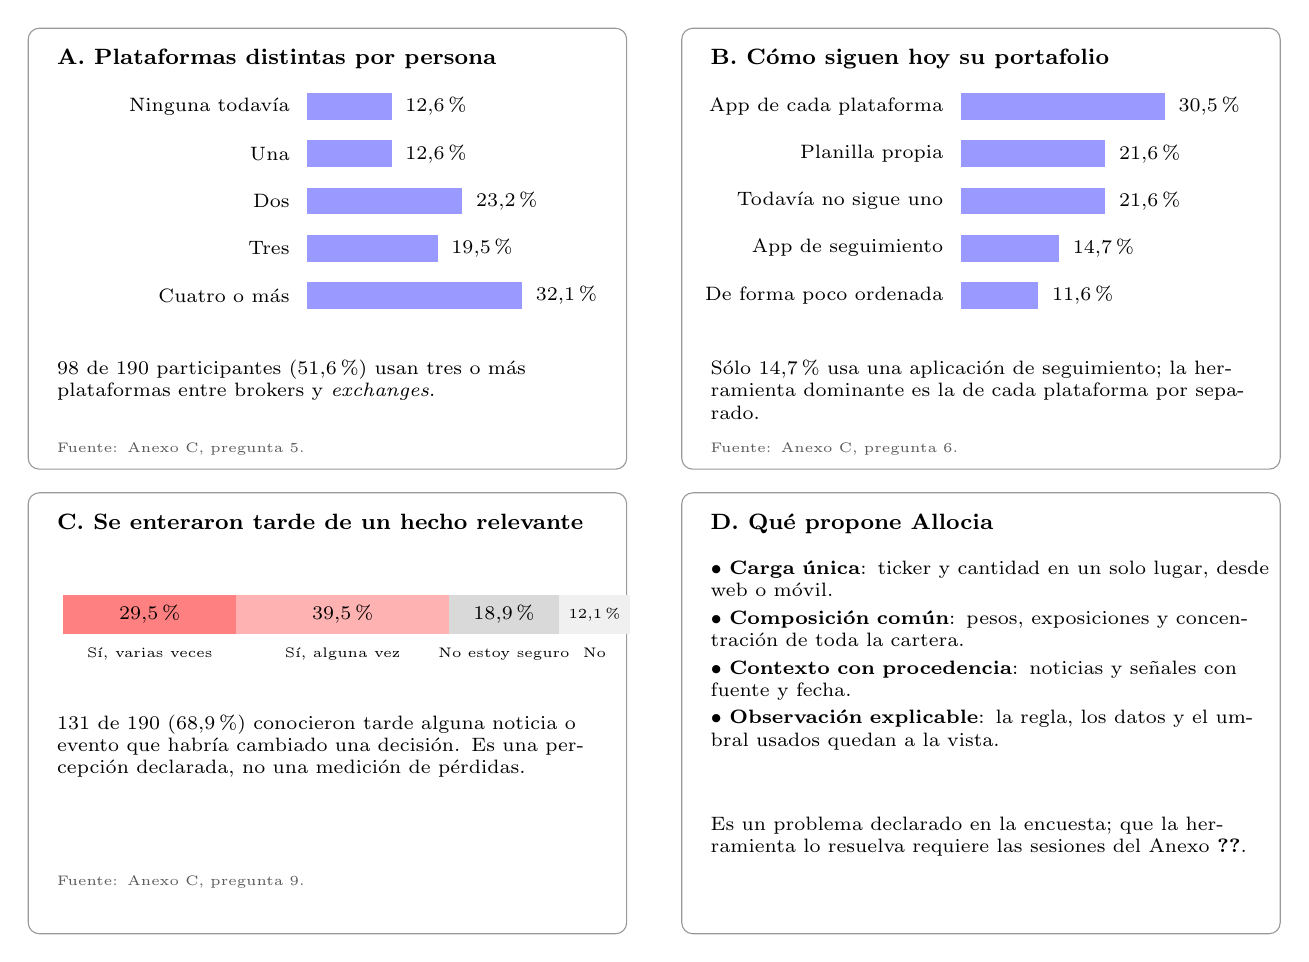
\begin{tikzpicture}[font=\scriptsize,
  panel/.style={draw=black!40,rounded corners,fill=white,minimum width=7.6cm,minimum height=5.6cm,anchor=north west},
  ttl/.style={font=\footnotesize\bfseries,anchor=north west},
  lab/.style={anchor=east,text width=3.2cm,align=right,font=\scriptsize},
  val/.style={anchor=west,font=\scriptsize},
  par/.style={anchor=north west,text width=7.1cm},
  src/.style={anchor=south west,font=\tiny,text=black!65,text width=7.1cm}]
%% Panel A: plataformas
\node[panel] at (0,0) {};
\node[ttl] at (0.25,-0.15) {A. Plataformas distintas por persona};
\begin{scope}[shift={(0.25,0)}]
\foreach \y/\n/\v/\t in {-1.0/Ninguna todavía/12.6/12{,}6, -1.6/Una/12.6/12{,}6, -2.2/Dos/23.2/23{,}2, -2.8/Tres/19.5/19{,}5, -3.4/Cuatro o más/32.1/32{,}1}{
  \node[lab] at (3.2,\y) {\n};\fill[blue!40] (3.3,\y-0.17) rectangle ({3.3+\v*0.085},\y+0.17);\node[val] at ({3.35+\v*0.085},\y) {\t\,\%};}
\end{scope}
\node[par] at (0.25,-4.1) {98 de 190 participantes (51{,}6\,\%) usan tres o más plataformas entre brokers y \textit{exchanges}.};
\node[src] at (0.25,-5.55) {Fuente: Anexo C, pregunta 5.};
%% Panel B: seguimiento
\node[panel] at (8.3,0) {};
\node[ttl] at (8.55,-0.15) {B. Cómo siguen hoy su portafolio};
\begin{scope}[shift={(8.55,0)}]
\foreach \y/\n/\v/\t in {-1.0/App de cada plataforma/30.5/30{,}5, -1.6/Planilla propia/21.6/21{,}6, -2.2/Todavía no sigue uno/21.6/21{,}6, -2.8/App de seguimiento/14.7/14{,}7, -3.4/De forma poco ordenada/11.6/11{,}6}{
  \node[lab] at (3.2,\y) {\n};\fill[blue!40] (3.3,\y-0.17) rectangle ({3.3+\v*0.085},\y+0.17);\node[val] at ({3.35+\v*0.085},\y) {\t\,\%};}
\end{scope}
\node[par] at (8.55,-4.1) {Sólo 14{,}7\,\% usa una aplicación de seguimiento; la herramienta dominante es la de cada plataforma por separado.};
\node[src] at (8.55,-5.55) {Fuente: Anexo C, pregunta 6.};
%% Panel C: enterarse tarde
\node[panel] at (0,-5.9) {};
\node[ttl] at (0.25,-6.05) {C. Se enteraron tarde de un hecho relevante};
\begin{scope}[shift={(0.25,-5.9)}]
\fill[red!50] (0.2,-1.3) rectangle (2.4,-1.8);\node[font=\scriptsize] at (1.3,-1.55) {29{,}5\,\%};
\fill[red!30] (2.4,-1.3) rectangle (5.1,-1.8);\node[font=\scriptsize] at (3.75,-1.55) {39{,}5\,\%};
\fill[black!15] (5.1,-1.3) rectangle (6.5,-1.8);\node[font=\scriptsize] at (5.8,-1.55) {18{,}9\,\%};
\fill[black!6] (6.5,-1.3) rectangle (7.4,-1.8);\node[font=\tiny] at (6.95,-1.55) {12{,}1\,\%};
\node[font=\tiny,anchor=north] at (1.3,-1.85) {Sí, varias veces};
\node[font=\tiny,anchor=north] at (3.75,-1.85) {Sí, alguna vez};
\node[font=\tiny,anchor=north] at (5.8,-1.85) {No estoy seguro};
\node[font=\tiny,anchor=north] at (6.95,-1.85) {No};
\end{scope}
\node[par] at (0.25,-8.6) {131 de 190 (68{,}9\,\%) conocieron tarde alguna noticia o evento que habría cambiado una decisión. Es una percepción declarada, no una medición de pérdidas.};
\node[src] at (0.25,-11.05) {Fuente: Anexo C, pregunta 9.};
%% Panel D: respuesta de diseño
\node[panel] at (8.3,-5.9) {};
\node[ttl] at (8.55,-6.05) {D. Qué propone Allocia};
\node[par] at (8.55,-6.65) {$\bullet$ \textbf{Carga única}: ticker y cantidad en un solo lugar, desde web o móvil.\\[2pt]
$\bullet$ \textbf{Composición común}: pesos, exposiciones y concentración de toda la cartera.\\[2pt]
$\bullet$ \textbf{Contexto con procedencia}: noticias y señales con fuente y fecha.\\[2pt]
$\bullet$ \textbf{Observación explicable}: la regla, los datos y el umbral usados quedan a la vista.};
\node[par] at (8.55,-9.9) {Es un problema declarado en la encuesta; que la herramienta lo resuelva requiere las sesiones del Anexo~\ref{annex:protocolo-usuarios}.};
\end{tikzpicture}
\caption{El problema del inversor con activos en varias plataformas según la encuesta (N=190). Fuente: elaboración propia.}\label{fig:problema-cifras}
\end{figure}


El problema delimitado es el esfuerzo de consolidación e interpretación de la cartera. Que lo experimente toda persona inversora, o que una explicación automatizada mejore sus resultados financieros, son cuestiones que el Proyecto no aborda.

\section{Necesidad que busca resolver el Proyecto}\label{sec:necesidad}

La necesidad consiste en disponer de una vista común que muestre composición y exposición, relacione señales con las posiciones y permita inspeccionar la evidencia de cada observación. La decisión corresponde al usuario; la herramienta organiza información y muestra las condiciones de sus reglas.

Las entrevistas muestran con qué sustitutos se cubre hoy esa necesidad (Subsubsección~\ref{subsec:entrevistas}): una planilla o un sitio de seguimiento general como Yahoo Finance para consolidar manualmente las posiciones, la aplicación del intermediario para cada cuenta y herramientas de IA de propósito general para leer noticias o revisar la cartera. Ninguno de esos sustitutos ofrece, por sí solo, una composición común de activos de distintas plataformas con la regla y la fuente de cada observación a la vista; esa es la tarea que Allocia propone resolver. La comparación proviene del relato de dos entrevistados, no de una evaluación de cada herramienta.

\section{Solución propuesta}\label{sec:solucion}

Allocia organiza un catálogo de instrumentos, posiciones ingresadas manualmente, métricas de composición y un motor de observaciones explicables. El usuario identifica cada instrumento por su ticker, un símbolo de mercado como AAPL, y registra su cantidad. El sistema calcula el valor con el precio del instrumento (el de referencia del catálogo o, en el servicio publicado, la cotización verificada) y deriva pesos y exposiciones. Ese conjunto acotado de funciones constituye el producto mínimo viable (MVP): la versión más reducida que permite evaluar si la propuesta resulta útil.

La plataforma ofrece dos clientes sobre la misma cuenta y la misma API: la aplicación web, para computadoras y para teléfonos sin la aplicación instalada, y la aplicación móvil nativa, orientada al uso cotidiano desde el teléfono. El repositorio contiene ambos clientes. Los dos incorporan registro, inicio y cierre de sesión y envío de la credencial a la API; su recorrido integrado se verifica en la Sección~\ref{chap:pruebas}. El cliente móvil responde a un hábito relevado: 86 de 190 participantes (45,3\,\%) siguen sus inversiones con aplicaciones, sea la de cada plataforma o una de seguimiento (Subsubsección~\ref{subsec:encuesta}). Como la encuesta preguntó por una plataforma web, se mantienen ambos clientes en lugar de reemplazar la web por la aplicación móvil. La Figura~\ref{fig:flujo-valor} resume el recorrido desde las posiciones dispersas en varias plataformas hasta la observación explicable.
% Infografía: del inversor con activos dispersos a la observación explicable.
\begin{figure}[ht]\centering
\begin{tikzpicture}[
  font=\scriptsize,
  stp/.style={draw,rounded corners,align=center,text width=2.2cm,minimum height=1.9cm,inner sep=4pt,fill=blue!5},
  src/.style={draw,rounded corners,align=center,text width=1.9cm,minimum height=0.6cm,inner sep=2pt,fill=black!4,font=\scriptsize},
  note/.style={align=center,text width=2.6cm,font=\scriptsize,text=black!70},
  arr/.style={-{Stealth},thick}]
\node[stp] (s1) {\textbf{1. Inversor}\\Posiciones repartidas en varias plataformas};
\node[stp,right=0.26cm of s1] (s2) {\textbf{2. Carga}\\Ticker y cantidad en Allocia (web o móvil)};
\node[stp,right=0.26cm of s2,fill=orange!8] (s3) {\textbf{3. Integración}\\Catálogo, cotizaciones fechadas y señales con procedencia};
\node[stp,right=0.26cm of s3] (s4) {\textbf{4. Análisis}\\Pesos, exposiciones, HHI y posiciones efectivas};
\node[stp,right=0.26cm of s4,fill=green!8] (s5) {\textbf{5. Observación}\\Regla + métricas + evidencia};
\foreach \a/\b in {s1/s2,s2/s3,s3/s4,s4/s5}\draw[arr] (\a)--(\b);
% Orígenes dispersos que alimentan la carga
\node[src,above=0.95cm of s1] (p2) {Intermediario local};
\node[src,left=0.15cm of p2,xshift=-0.1cm] (p1) {Exchange cripto};
\node[src,right=0.15cm of p2,xshift=0.1cm] (p3) {Planilla propia};
\foreach \p in {p1,p2,p3}\draw[arr,black!50] (\p.south)--(s1.north);
% Qué recibe el usuario
\node[note,below=0.35cm of s5] (u) {El usuario revisa la condición activada y decide; la herramienta no opera ni recomienda comprar o vender.};
\node[note,below=0.35cm of s3] (n3) {Cada dato conserva fuente, fecha y condición (en vivo o demostración).};
\node[note,below=0.35cm of s1] (n1) {Situación descripta en la encuesta y en las entrevistas.};
\end{tikzpicture}
\caption{De los activos dispersos a la observación explicable. Fuente: elaboración propia.}\label{fig:flujo-valor}
\end{figure}


Las observaciones muestran la condición activada y su evidencia; cuando intervienen datos locales de demostración, esa condición se indica. El sistema también genera informes por activo con un modelo de lenguaje restringido a fuentes públicas citadas, con los controles de la Subsección~\ref{sec:seguridad}. Allocia no pronostica rendimientos ni ejecuta operaciones.

\section{Modelo de negocio}\label{sec:modelo-negocio}

El modelo de negocio describe cómo Allocia podría sostenerse más allá del Proyecto académico. La Figura~\ref{fig:canvas} lo resume con el lienzo de modelo de negocio \parencite{Osterwalder2010}; los párrafos siguientes detallan los bloques que dependen de la investigación con usuarios y del relevamiento de proveedores.
% Lienzo de modelo de negocio (Osterwalder y Pigneur) de Allocia.
\begin{figure}[ht]\centering
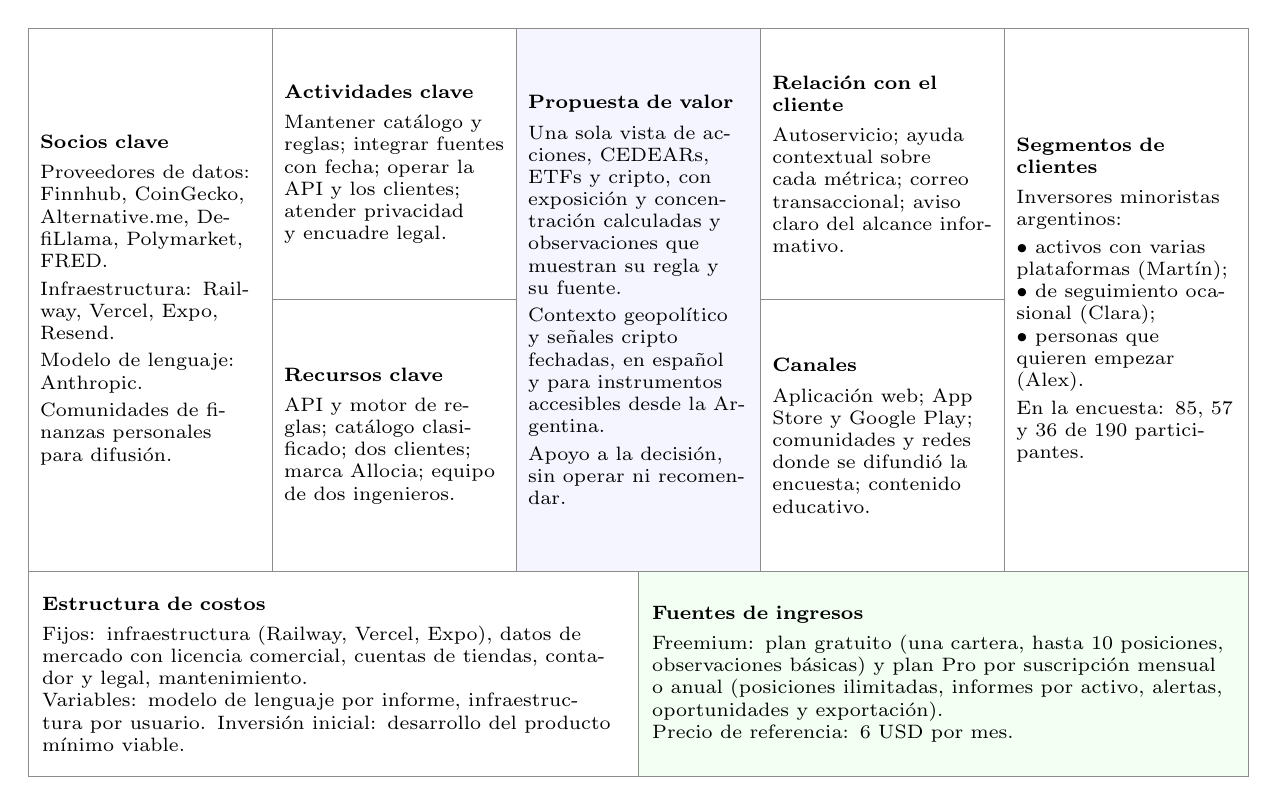
\begin{tikzpicture}[font=\scriptsize,
  blk/.style={draw=black!45,fill=white,inner sep=4pt,align=left,anchor=north west},
  t/.style={font=\scriptsize\bfseries}]
\def\w{3.1}\def\hh{6.9}\def\hl{2.6}
\node[blk,minimum width=\w cm,minimum height=\hh cm,text width=2.8cm] at (0,0) {\textbf{Socios clave}\\[3pt]Proveedores de datos: Finnhub, CoinGecko, Alternative.me, DefiLlama, Polymarket, FRED.\\[2pt]Infraestructura: Railway, Vercel, Expo, Resend.\\[2pt]Modelo de lenguaje: Anthropic.\\[2pt]Comunidades de finanzas personales para difusión.};
\node[blk,minimum width=\w cm,minimum height=3.45cm,text width=2.8cm] at (\w,0) {\textbf{Actividades clave}\\[3pt]Mantener catálogo y reglas; integrar fuentes con fecha; operar la API y los clientes; atender privacidad y encuadre legal.};
\node[blk,minimum width=\w cm,minimum height=3.45cm,text width=2.8cm] at (\w,-3.45) {\textbf{Recursos clave}\\[3pt]API y motor de reglas; catálogo clasificado; dos clientes; marca Allocia; equipo de dos ingenieros.};
\node[blk,minimum width=\w cm,minimum height=\hh cm,text width=2.8cm,fill=blue!4] at (2*\w,0) {\textbf{Propuesta de valor}\\[3pt]Una sola vista de acciones, CEDEARs, ETFs y cripto, con exposición y concentración calculadas y observaciones que muestran su regla y su fuente.\\[2pt]Contexto geopolítico y señales cripto fechadas, en español y para instrumentos accesibles desde la Argentina.\\[2pt]Apoyo a la decisión, sin operar ni recomendar.};
\node[blk,minimum width=\w cm,minimum height=3.45cm,text width=2.8cm] at (3*\w,0) {\textbf{Relación con el cliente}\\[3pt]Autoservicio; ayuda contextual sobre cada métrica; correo transaccional; aviso claro del alcance informativo.};
\node[blk,minimum width=\w cm,minimum height=3.45cm,text width=2.8cm] at (3*\w,-3.45) {\textbf{Canales}\\[3pt]Aplicación web; App Store y Google Play; comunidades y redes donde se difundió la encuesta; contenido educativo.};
\node[blk,minimum width=\w cm,minimum height=\hh cm,text width=2.8cm] at (4*\w,0) {\textbf{Segmentos de clientes}\\[3pt]Inversores minoristas argentinos:\\[2pt]$\bullet$ activos con varias plataformas (Martín);\\$\bullet$ de seguimiento ocasional (Clara);\\$\bullet$ personas que quieren empezar (Alex).\\[2pt]En la encuesta: 85, 57 y 36 de 190 participantes.};
\node[blk,minimum width=2.5*\w cm,minimum height=\hl cm,text width=7.4cm] at (0,-\hh) {\textbf{Estructura de costos}\\[3pt]Fijos: infraestructura (Railway, Vercel, Expo), datos de mercado con licencia comercial, cuentas de tiendas, contador y legal, mantenimiento.\\Variables: modelo de lenguaje por informe, infraestructura por usuario. Inversión inicial: desarrollo del producto mínimo viable.};
\node[blk,minimum width=2.5*\w cm,minimum height=\hl cm,text width=7.4cm,fill=green!5] at (2.5*\w,-\hh) {\textbf{Fuentes de ingresos}\\[3pt]Freemium: plan gratuito (una cartera, hasta 10 posiciones, observaciones básicas) y plan Pro por suscripción mensual o anual (posiciones ilimitadas, informes por activo, alertas, oportunidades y exportación).\\Precio de referencia: 6 USD por mes.};
\end{tikzpicture}
\caption{Lienzo del modelo de negocio de Allocia. Fuente: elaboración propia a partir del lienzo de modelo de negocio \parencite{Osterwalder2010}.}\label{fig:canvas}
\end{figure}


Los segmentos son los tres arquetipos de la Subsubsección~\ref{subsec:user-persona}: inversores activos con posiciones en varias plataformas, inversores de seguimiento ocasional y personas que quieren empezar. La propuesta de valor para los tres es una única vista de la cartera con exposición y concentración calculadas, contexto fechado y observaciones que muestran su regla y su fuente. Para el inversor activo, el valor está en el tiempo que ahorra la consolidación y en la alerta temprana; para el ocasional, en un resumen comprensible; para quien empieza, en las definiciones visibles y en el límite claro entre información y recomendación.

El ingreso previsto es una suscripción freemium. El plan gratuito admite una cartera de hasta diez posiciones con composición, concentración y observaciones básicas; el plan Pro agrega posiciones ilimitadas, informes por activo con fuentes, alertas, seguimiento de activos no poseídos y exportación. La encuesta respalda esa estructura: el 50,0\,\% de los participantes usaría la herramienta solo si tiene una versión gratuita con funciones pagas, el 25,8\,\% pagaría una suscripción mensual, el 15,8\,\% la usaría solo si es gratis y el 8,4\,\% no la usaría (Anexo~\ref{annex:user-research}). Esas respuestas expresan intención, no pago efectivo. El precio de referencia del plan Pro es 6 dólares por mes, por debajo del plan inicial de Sharesight (9,33 dólares) y del plan anual de Kubera (unos 20,8 dólares por mes) y en el rango de CoinStats Premium \parencite{SharesightPricing,KuberaPricing,CoinStatsPricing}.

Los canales son la aplicación web, las tiendas de aplicaciones y las comunidades de finanzas personales donde se difundió la encuesta. La relación con el cliente es de autoservicio, con ayuda contextual, correo transaccional y un aviso permanente sobre el alcance informativo del producto. Los socios clave son los proveedores de datos, de infraestructura y del modelo de lenguaje; varios de ellos condicionan el uso comercial: Finnhub ofrece el plan gratuito solo para uso personal, FRED pide consentimiento escrito para uso comercial y Vercel reserva el plan gratuito a proyectos no comerciales \parencite{FinnhubPricing,FredTerms,VercelPricing}. Un servicio pago necesita los planes correspondientes, que la Subsección~\ref{sec:viabilidad} incorpora a los costos.

Dos restricciones delimitan el modelo. La primera es legal: Allocia no está inscripta como agente ante la CNV, por lo que no puede prestar asesoramiento habitual y profesional ni ejecutar operaciones (Subsubsección~\ref{subsec:marco-normativo}); el plan Pro vende análisis e información, no consejo personalizado. La segunda es tributaria: el precio se expresa sin IVA, cuya alícuota general es del 21\,\% \parencite{LeyIVA}, y la forma societaria condiciona el régimen: una sociedad tributa en el régimen general, mientras que el monotributo solo alcanza a personas humanas \parencite{LeyMonotributo}.

\section{Viabilidad económico-financiera}\label{sec:viabilidad}

La viabilidad se evalúa con un flujo de fondos mensual a 36 meses, en dólares y sin IVA, con tres escenarios y las herramientas de valor actual neto (VAN), tasa interna de retorno (TIR), período de recupero y punto de equilibrio. El cálculo se reproduce con el script \texttt{scripts/viabilidad.py} del repositorio del Proyecto. La Tabla~\ref{tab:supuestos} reúne los supuestos; los precios provienen de las páginas oficiales de los proveedores, consultadas el 22 de octubre de 2026 \parencite{RailwayPricing,VercelPricing,ExpoPricing,FinnhubPricing,CoinGeckoPricing,ResendPricing,AppleDeveloper,GooglePlayConsole,AnthropicPricing}.

\begin{table}[ht]
\centering\small\renewcommand{\arraystretch}{1.15}
\caption{Supuestos del flujo de fondos. Fuente: elaboración propia a partir de las páginas oficiales de los proveedores.}\label{tab:supuestos}
\begin{tabular}{>{\raggedright\arraybackslash}p{6.4cm}>{\raggedright\arraybackslash}p{7.2cm}}\hline
\textbf{Concepto} & \textbf{Valor}\\\hline
Inversión inicial & 10\,324 USD: desarrollo del MVP (dos personas, ocho meses, 40 horas mensuales a 15 USD la hora), cuentas de Apple (99 USD) y Google Play (25 USD), marca y asesoramiento legal (600 USD).\\
Costos fijos mensuales & 517 USD: Railway (40), Vercel Pro (20), Expo Starter (19), datos de mercado Finnhub (50), Apple prorrateado (8), contador y legal (80), mantenimiento y soporte (20 horas a 15 USD).\\
Costos escalonados & Resend Pro (20 USD) a partir de 3\,000 usuarios registrados; CoinGecko Analyst (129 USD) a partir de 300 usuarios Pro.\\
Costo variable & 1 USD por usuario Pro y mes (informes con el modelo de lenguaje, unos 30 por mes a 0,03 USD, más infraestructura) y 0,02 USD por usuario registrado.\\
Ingreso & 6 USD por usuario Pro y mes.\\
Escenario pesimista & 150 registros por mes; conversión a Pro del 2\,\%; baja mensual del 6\,\%; marketing 150 USD.\\
Escenario base & 300 registros por mes; conversión del 4\,\%; baja del 5\,\%; marketing 200 USD.\\
Escenario optimista & 600 registros por mes; conversión del 6\,\%; baja del 4\,\%; marketing 300 USD.\\
Tasa de descuento & 20\,\% anual (1,53\,\% mensual).\\
Simplificaciones & Sin impuesto a las ganancias ni ingresos brutos; sin remuneración de los fundadores más allá del mantenimiento; abandono del 3\,\% mensual de usuarios registrados.\\\hline
\end{tabular}
\end{table}

La conversión supuesta es una fracción de la intención declarada: el 25,8\,\% que dice que pagaría se reduce a entre el 2\,\% y el 6\,\% de los registrados, en línea con la diferencia habitual entre intención y pago. La Tabla~\ref{tab:resultados-viabilidad} presenta los resultados y la Figura~\ref{fig:flujo-caja} el flujo de caja acumulado.

\begin{table}[ht]
\centering\small\renewcommand{\arraystretch}{1.15}
\caption{Resultados a 36 meses por escenario. Fuente: elaboración propia.}\label{tab:resultados-viabilidad}
\begin{tabular}{>{\raggedright\arraybackslash}p{5.6cm}rrr}\hline
\textbf{Indicador} & \textbf{Pesimista} & \textbf{Base} & \textbf{Optimista}\\\hline
Punto de equilibrio mensual (usuarios Pro) & 133 & 143 & 163\\
Usuarios Pro en el mes 36 & 45 & 202 & 693\\
Ingreso mensual en el mes 36 (USD) & 268 & 1\,213 & 4\,158\\
Costo mensual en el mes 36 (USD) & 798 & 1\,073 & 1\,926\\
Primer mes con flujo operativo positivo & no alcanza & 25 & 7\\
Período de recupero de la inversión & no alcanza & más de 36 meses & 21 meses\\
VAN a 36 meses, 20\,\% anual (USD) & $-25\,829$ & $-15\,300$ & $16\,284$\\
TIR anual & no existe & negativa & 87,8\,\%\\\hline
\end{tabular}
\end{table}
% Flujo de caja acumulado por escenario (USD), generado por scripts/viabilidad.py
\begin{figure}[ht]\centering
\begin{tikzpicture}[font=\scriptsize]
\draw[black!50] (0,3.13)--(12.5,3.13);
\draw[-{Stealth}] (0,0)--(0,6.3);\draw[-{Stealth}] (0,0)--(12.8,0);
\draw[black!25,dotted] (0,0.45)--(12.5,0.45);\node[anchor=east] at (-0.1,0.45) {-30\,000};
\draw[black!25,dotted] (0,1.34)--(12.5,1.34);\node[anchor=east] at (-0.1,1.34) {-20\,000};
\draw[black!25,dotted] (0,2.24)--(12.5,2.24);\node[anchor=east] at (-0.1,2.24) {-10\,000};
\draw[black!25,dotted] (0,3.13)--(12.5,3.13);\node[anchor=east] at (-0.1,3.13) {0\,000};
\draw[black!25,dotted] (0,4.03)--(12.5,4.03);\node[anchor=east] at (-0.1,4.03) {10\,000};
\draw[black!25,dotted] (0,4.93)--(12.5,4.93);\node[anchor=east] at (-0.1,4.93) {20\,000};
\draw[black!25,dotted] (0,5.82)--(12.5,5.82);\node[anchor=east] at (-0.1,5.82) {30\,000};
\node[anchor=north] at (2.08,-0.05) {6};
\node[anchor=north] at (4.17,-0.05) {12};
\node[anchor=north] at (6.25,-0.05) {18};
\node[anchor=north] at (8.33,-0.05) {24};
\node[anchor=north] at (10.42,-0.05) {30};
\node[anchor=north] at (12.50,-0.05) {36};
\node[anchor=north] at (6.25,-0.45) {Mes};\node[rotate=90,anchor=south] at (-1.1,3.00) {Flujo de caja acumulado (USD)};
\draw[red!70,thick] (0,2.21) -- (0.35,2.15) -- (0.69,2.09) -- (1.04,2.04) -- (1.39,1.98) -- (1.74,1.93) -- (2.08,1.87) -- (2.43,1.82) -- (2.78,1.76) -- (3.12,1.71) -- (3.47,1.66) -- (3.82,1.61) -- (4.17,1.56) -- (4.51,1.51) -- (4.86,1.46) -- (5.21,1.41) -- (5.56,1.36) -- (5.90,1.31) -- (6.25,1.26) -- (6.60,1.21) -- (6.94,1.17) -- (7.29,1.12) -- (7.64,1.07) -- (7.99,1.02) -- (8.33,0.98) -- (8.68,0.93) -- (9.03,0.88) -- (9.38,0.84) -- (9.72,0.79) -- (10.07,0.74) -- (10.42,0.70) -- (10.76,0.65) -- (11.11,0.60) -- (11.46,0.55) -- (11.81,0.51) -- (12.15,0.46) -- (12.50,0.41);
\node[anchor=west,red!70] at (12.55,0.41) {Pesimista};
\draw[orange!85!black,thick] (0,2.21) -- (0.35,2.15) -- (0.69,2.10) -- (1.04,2.05) -- (1.39,2.00) -- (1.74,1.96) -- (2.08,1.92) -- (2.43,1.88) -- (2.78,1.85) -- (3.12,1.82) -- (3.47,1.80) -- (3.82,1.77) -- (4.17,1.75) -- (4.51,1.73) -- (4.86,1.71) -- (5.21,1.70) -- (5.56,1.69) -- (5.90,1.68) -- (6.25,1.67) -- (6.60,1.66) -- (6.94,1.65) -- (7.29,1.65) -- (7.64,1.65) -- (7.99,1.65) -- (8.33,1.65) -- (8.68,1.65) -- (9.03,1.65) -- (9.38,1.66) -- (9.72,1.66) -- (10.07,1.67) -- (10.42,1.68) -- (10.76,1.69) -- (11.11,1.70) -- (11.46,1.71) -- (11.81,1.72) -- (12.15,1.73) -- (12.50,1.74);
\node[anchor=west,orange!85!black] at (12.55,1.74) {Base};
\draw[green!55!black,thick] (0,2.21) -- (0.35,2.15) -- (0.69,2.11) -- (1.04,2.08) -- (1.39,2.06) -- (1.74,2.06) -- (2.08,2.06) -- (2.43,2.08) -- (2.78,2.11) -- (3.12,2.15) -- (3.47,2.19) -- (3.82,2.24) -- (4.17,2.30) -- (4.51,2.37) -- (4.86,2.44) -- (5.21,2.53) -- (5.56,2.62) -- (5.90,2.72) -- (6.25,2.83) -- (6.60,2.95) -- (6.94,3.07) -- (7.29,3.20) -- (7.64,3.33) -- (7.99,3.47) -- (8.33,3.62) -- (8.68,3.77) -- (9.03,3.93) -- (9.38,4.09) -- (9.72,4.26) -- (10.07,4.43) -- (10.42,4.61) -- (10.76,4.79) -- (11.11,4.97) -- (11.46,5.16) -- (11.81,5.35) -- (12.15,5.55) -- (12.50,5.75);
\node[anchor=west,green!55!black] at (12.55,5.75) {Optimista};
\end{tikzpicture}
\caption{Flujo de caja acumulado a 36 meses por escenario, en dólares y sin IVA. Fuente: elaboración propia con scripts/viabilidad.py.}\label{fig:flujo-caja}
\end{figure}

El punto de equilibrio operativo está entre 133 y 163 usuarios Pro, según el gasto de marketing: con una contribución de 5 dólares por usuario, esa cantidad cubre los costos fijos. El escenario pesimista no lo alcanza: la combinación de pocos registros y baja conversión estabiliza la base paga en unos 50 usuarios. El escenario base cruza el equilibrio operativo en el mes 25, pero no recupera la inversión inicial dentro de los 36 meses. El escenario optimista recupera la inversión en el mes 21 y obtiene un VAN positivo con una TIR del 87,8\,\% anual.

La sensibilidad al precio es alta. Con un plan Pro de 9 dólares, cercano a Sharesight, el punto de equilibrio del escenario base baja a 90 usuarios y el VAN se acerca a cero ($-5\,003$ USD), mientras que el escenario optimista recupera la inversión en el mes 14. En sentido contrario, un plan comercial de datos de mercado más caro que el supuesto (el plan para empresas de Finnhub no publica precio) desplaza el equilibrio hacia arriba.

La conclusión es que el producto es viable como negocio solo si la adquisición y la conversión se aproximan al escenario optimista o si el precio se ubica en el rango de los competidores. Esas dos variables no se conocen: la encuesta mide intención y la aplicación no se ofreció al público. Por eso, validar la disposición a pagar con usuarios reales, con una lista de espera y un plan Pro de prueba, es la primera actividad del plan de negocio después del cierre académico. Mientras tanto, el prototipo opera con costos cercanos a cero sobre los planes gratuitos, que alcanzan para el uso del equipo y para las sesiones de evaluación.

\section{Requerimientos funcionales}\label{sec:req-funcionales}

Los doce requerimientos funcionales se identifican de RF1 a RF12 y cada uno se formula como un comportamiento verificable del sistema:
\begin{enumerate}[label=RF\arabic*.,leftmargin=*]
\item El sistema debe permitir el registro y el inicio de sesión, y asociar las posiciones a la cuenta autenticada.
\item El sistema debe permitir cargar, editar y eliminar posiciones propias mediante ticker de catálogo y cantidad positiva, rechazando entradas inválidas.
\item El sistema debe clasificar las posiciones por clase, sector, región y moneda según el catálogo y mostrar el origen de esa clasificación.
\item El sistema debe calcular el valor de la cartera, pesos, exposiciones, HHI y número efectivo de posiciones, y tratar explícitamente una cartera vacía.
\item El sistema debe presentar contexto geopolítico y señales emergentes con fuente, fecha y condición de dato en vivo o de demostración por componente.
\item El sistema debe generar observaciones que incluyan regla, métricas y evidencia, y permitan inspeccionar su fundamento.
\item El sistema debe ofrecer el flujo de gestión y análisis de posiciones desde el cliente web y desde el cliente móvil, con una misma cuenta y los mismos contratos de API, y documentar las diferencias de funciones entre ambos clientes.
\item El sistema debe mostrar escenarios como simulaciones con supuestos visibles, sin presentarlos como predicciones.
\item El sistema debe permitir solicitar la eliminación de la cuenta y de sus posiciones mediante una confirmación explícita, informando el alcance de la eliminación.
\item El sistema debe informar finalidad, datos tratados, conservación y canales de ejercicio de derechos antes de registrar una cuenta, y registrar el consentimiento cuando corresponda.
\item El sistema debe generar informes por activo con un modelo de lenguaje a partir de un conjunto delimitado de fuentes públicas, validar su esquema y la coincidencia literal de cada cita con su fuente, y abstenerse cuando falten datos o las fuentes no estén vigentes, sin enviar identidad ni cantidades al proveedor.
\item El sistema debe separar los análisis de la cartera de las oportunidades sobre activos no poseídos, permitir seguir activos sin modificar tenencias y configurar alertas independientes de escenarios alcistas respaldados, informando cobertura, fechas, condiciones y riesgos sin atribuir probabilidades no calculadas.
\end{enumerate}

\section{Requerimientos no funcionales}\label{sec:req-no-funcionales}

Los siguientes umbrales son criterios de aceptación propuestos para el prototipo; cada evaluación registra entorno, procedimiento y resultados.
\begin{enumerate}[label=RNF\arabic*.,leftmargin=*]
\item El sistema debe presentar la interfaz en español, definir las métricas en lenguaje accesible y permitir que al menos cuatro de cinco participantes de una evaluación exploratoria identifiquen la causa de una observación sin ayuda. Ese tamaño de evaluación no permite generalización estadística.
\item El sistema debe producir pesos con error absoluto máximo de $10^{-6}$ frente a un cálculo independiente antes del redondeo, para carteras de prueba con valor positivo.
\item El sistema debe responder al análisis de hasta 100 posiciones en menos de dos segundos en el percentil 95 de 30 consultas con caché disponible, en un entorno documentado y sin incluir latencia de proveedores externos.
\item El sistema debe rechazar todas las solicitudes sin autenticación a datos privados y todas las modificaciones sobre posiciones ajenas en las pruebas de dos cuentas.
\item El sistema debe almacenar contraseñas mediante hash adaptativo, usar HTTPS en despliegues remotos y mantener secretos fuera del repositorio; debe documentar los controles de cifrado en reposo y copias de seguridad del proveedor.
\item El sistema debe mantener separados catálogo, posiciones, señales y observaciones, para permitir pruebas independientes de los cálculos y reglas.
\item El sistema debe identificar fallos o antigüedad de las fuentes y conservar la procedencia individual de los datos cuando combine proveedores y respaldo local.
\item El sistema debe limitarse al análisis informativo y a la presentación de evidencia, manteniendo las decisiones y operaciones financieras bajo control del usuario y fuera del flujo del prototipo.
\item El sistema debe contemplar minimización, acceso, rectificación y supresión de datos personales conforme al marco normativo aplicable, con evidencia verificable de los procedimientos.
\item El sistema debe indicar en la interfaz qué contenidos provienen del motor de reglas y cuáles fueron redactados por un modelo de lenguaje, y presentar ambos como apoyo informativo y no como asesoramiento de inversión.
\end{enumerate}

Los requerimientos no funcionales se corresponden con las características de una IA confiable \parencite{NIST2023airmf}: validez y fiabilidad (RNF2, RNF3 y RNF6), seguridad y resiliencia (RNF4, RNF5 y RNF7), explicabilidad e interpretabilidad (RNF1 y RNF10), privacidad (RNF9) y responsabilidad con supervisión humana (RNF8). La Subsección~\ref{sec:seguridad} detalla los controles asociados y su estado.

\section{Casos de uso principales}\label{sec:casos-uso}

La Figura~\ref{fig:casos-uso} presenta las interacciones previstas. La autenticación es precondición de las operaciones privadas y disponer de posiciones lo es del análisis; las posiciones guardadas no se vuelven a cargar en cada consulta del resumen.
\begin{figure}[ht]\centering
\begin{tikzpicture}[cu/.style={draw,ellipse,fill=blue!6,text width=5.4cm,align=center,font=\small,inner sep=4pt},line/.style={black!55}]
\node at (0,0) (actor) {Usuario};
\draw (0,0.6) circle (0.18);\draw (0,0.42)--(0,0.1);\draw (-0.25,0.3)--(0.25,0.3);
\foreach \y/\name/\txt in {4/cu8/{CU08: Registro e inicio de sesión},3/cu1/{CU01: Gestión de posiciones},2/cu2/{CU02: Resumen y composición},1/cu3/{CU03: Concentración},0/cu4/{CU04: Contexto y señales},-1/cu5/{CU05: Observaciones y evidencia},-2/cu6/{CU06: Escenarios},-3/cu7/{CU07: Detalle por activo},-4/cu9/{CU09: Baja de cuenta}}{
\node[cu] (\name) at (6,\y) {\txt};\draw[line] (actor.east)--(\name.west);}
\draw[rounded corners] (2.8,-4.6) rectangle (9.2,4.6);
\node[fill=white] at (6,4.6) {Allocia};
\end{tikzpicture}
\caption{Casos de uso previstos. Fuente: elaboración propia.}\label{fig:casos-uso}
\end{figure}


Los casos comprenden gestión de posiciones (CU01), resumen (CU02), concentración (CU03), señales (CU04), explicación (CU05), escenarios (CU06), detalle de activo (CU07), registro e inicio de sesión (CU08) y baja de cuenta (CU09). CU09 se implementa con reautenticación, confirmación, eliminación de posiciones y cuenta e invalidación de las sesiones anteriores. La Subsección~\ref{sec:validacion-publicada} presenta su verificación desde la web y el cliente HTTP móvil; la recepción push y la interacción en teléfonos físicos se validan por separado.

\section{Módulos del sistema}\label{sec:modulos}

La separación modular organiza responsabilidades y permite vincular cada requisito con su implementación o validación:
\begin{itemize}[nosep]
\item \textbf{Identidad y privacidad.} Registro, autenticación, autorización y ciclo de vida de la cuenta (RF1, RF9 y RF10).
\item \textbf{Catálogo y portafolio.} Clasificación y gestión de posiciones por propietario (RF2 y RF3).
\item \textbf{Análisis estructural.} Valores de referencia, pesos, exposiciones y concentración (RF4).
\item \textbf{Fuentes externas.} Normalización, procedencia, antigüedad y respaldo de señales (RF5).
\item \textbf{Observaciones.} Reglas deterministas y evidencia asociada; escenarios con supuestos explícitos (RF6 y RF8).
\item \textbf{Informes de análisis.} Redacción con modelo de lenguaje sobre fuentes públicas, con validación de esquema y de citas y abstención ante datos insuficientes (RF11).
\item \textbf{Presentación.} Cliente web y cliente móvil con contratos comunes (RF7).
\end{itemize}
